\chapter{PLANTEAMIENTO DEL PROBLEMA}
\section{Descripción de la Realidad Problemática}

El emprendimiento hoy en día es una realidad en todo el mundo. Desde crear productos nuevos hasta crear nuevas formas de hacer las cosas, todo gracias a ideas nacidas a partir de querer satisfacer nuestras propias necesidades.

Nuestro país no es ajeno a ello. El 50.6\% de la población entre 18 y 64 años tiene la expectativa de iniciar un emprendimiento dentro de los tres próximos años de acuerdo al último reporte de Global Entrepreneurship Monitor (GEM) 2014. El 62.3\% de la población entre ese rango de edad, además, tiende a ser más optimista en su percepción de oportunidades. Asimismo, según informa la Cámara de Comercio de Lima, la iniciativa emprendedora responde más a la identificación de una oportunidad de negocio que a una falta de oportunidad de empleo \parencite{cr_gestion2015emprendper}. Sin embargo, en un estudio más reciente basado en una encuesta realizada a residentes peruanos entre junio y julio del 2017 desarrollada por el equipo GEM Perú y ESAN a 2080 personas entre el mismo rango de edad, el 24.6\% de emprendimientos se encuentra en fase temprana, es decir, representa una dificultad para el emprendedor peruano llegar a etapas más avanzadas como un emprendimiento establecido (negocios con más de 3.5 años, que representan solo el 7.4\% para Perú), ubicando así a nuestro país en la posición 25 de 54 economías a nivel mundial \parencite{cr_gestion2018emprend}. En la Figura \ref{1:fig} se aprecian algunas ratios del estudio. %\medskip

\begin{figure}[h]
	\begin{center}
		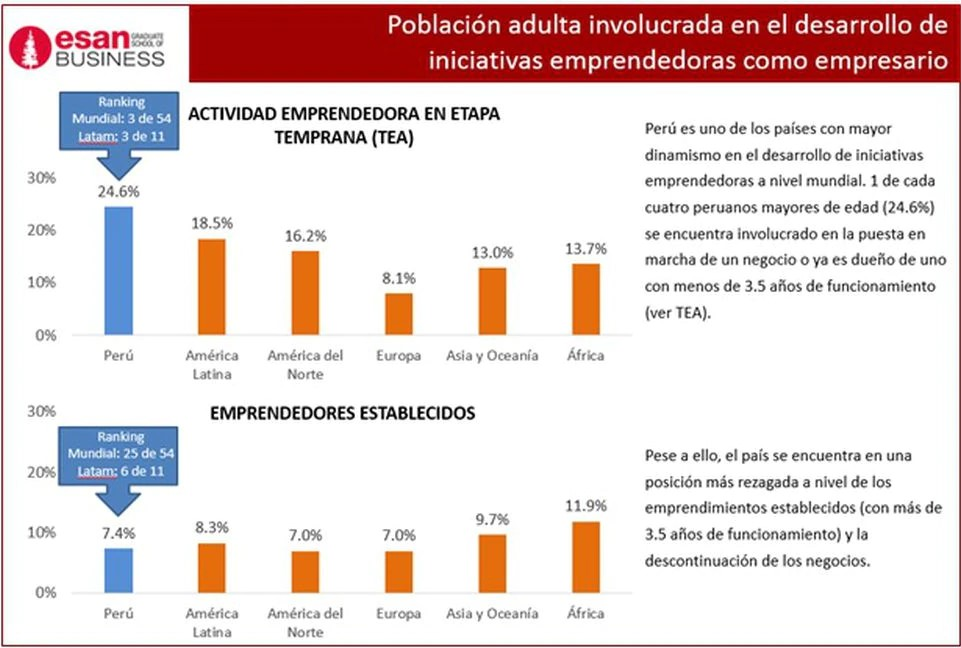
\includegraphics[width=0.7\textwidth]{1/figures/cuadro_esan.jpg}
		\caption{Resultados y ratios obtenidos en la encuesta por GEM y ESAN. Fuente: \cite{cr_gestion2018emprend}}
		\label{1:fig}
	\end{center}
\end{figure}

Estos resultados desfavorables tienen como base el ecosistema poco beneficioso para los emprendimientos que permitan su establecimiento en el entorno nacional, con condiciones asociadas al acceso de financiamiento, políticas gubernamentales que alienten la implementación de Innovación y Desarrollo en las empresas, acceso a infraestructura física y asesoría a nivel comercial y profesional, como sostiene el investigador del equipo GEM Perú Carlos Guerrero \parencite{cr_gestion2018emprend}. La Asociación de Emprendedores de Perú (ASEP) afirma, asimismo, que en la región solo se invierte el 1.5\% del PIB en actividades de ciencia, tecnología e innovación, y las limitaciones son dadas por barreras burocráticas ejercidas por el Gobierno y el sector privado \parencite{cr_aep2018emprend}. En adición a esto, otras razones que representan barreras para emprender son la falta de conocimientos en la iniciación de un negocio, su tramitación, la fuente de financiamiento del proyecto o búsqueda de inversionistas, la cultura, la falta de fomento de emprendimiento y la falta de una red de contactos \parencite{cr_sandoval_barreras}.

Ante estas limitaciones, en la actualidad muchos emprendedores se ven forzados a mostrar sus proyectos al público en la Internet con el fin de captar personas interesadas en ayudarlos en el financiamiento de estos. Por ello, se han creado plataformas web con el fin de permitir la interacción entre los proyectos publicados en un determinado tiempo, el cual puede variar entre 30 y 120 días, y la comunidad en general que desee colaborar con una cantidad de dinero para su financiamiento. El sitio web solo servirá para mostrar los proyectos presentados a detalle por los creadores y la promoción de estos al público. La idea es que, al término de este plazo de tiempo, el proyecto sea financiado y se logre convertir en una realidad. A esta práctica se le conoce como crowdfunding \parencite{cr_uc_crowdfunding}.

En Latinoamérica, son muy pocos los países los que se incorporan en el crowdfunding, tales como Chile, México, Argentina y Brasil. Sin embargo, el modelo funciona distinto a países de Norteamérica y Europa debido a la cultura diferente y resistencia a su implementación por la poca confianza en el éxito de los proyectos. En los últimos años se decidió seguir una manera muy similar a los modelos de Estados Unidos, basados en la creación de campañas de un emprendedor para obtener fondos para sus ideas con la moneda norteamericana pero limitados a las leyes económicas de cada país \parencite{cr_sl_crowdfundlatam}.

Entre los sitios web más conocidos de crowdfunding están Kickstarter e Indiegogo. Kickstarter, desde su inicio en 2009, es una plataforma de financiamiento de proyectos creativos de todo tipo, los cuales incluyen películas, juegos, música, arte, diseño y tecnología. Actualmente, se han registrado más de 162 mil proyectos realizados, 16 millones de contribuyentes y 4,3 miles de millones de dólares fondeados \parencite{cr_kickstarter_about}. La plataforma utiliza un modelo de financiamiento llamado “todo o nada”, el cual consiste en que si un proyecto no alcanza su meta de financiamiento en un determinado plazo de tiempo, no se realiza ninguna transacción de fondos \parencite{cr_kickstarter_founding}. Si bien los patrocinadores apoyan estos proyectos por motivos personales y distintos para hacerlos realidad, ellos no obtienen la propiedad o los ingresos de los proyectos que financian, sino que los creadores conservan la totalidad de su trabajo \parencite{cr_kickstarter_press}.

Para los proyectos tecnológicos, en contraste, la ratio de éxito es uno de los más bajos de las categorías existentes (20\%) solo por delante de Artesanía y Periodismo, como se aprecia en la Figura \ref{1:fig2}.
\begin{figure}[h]
	\begin{center}
		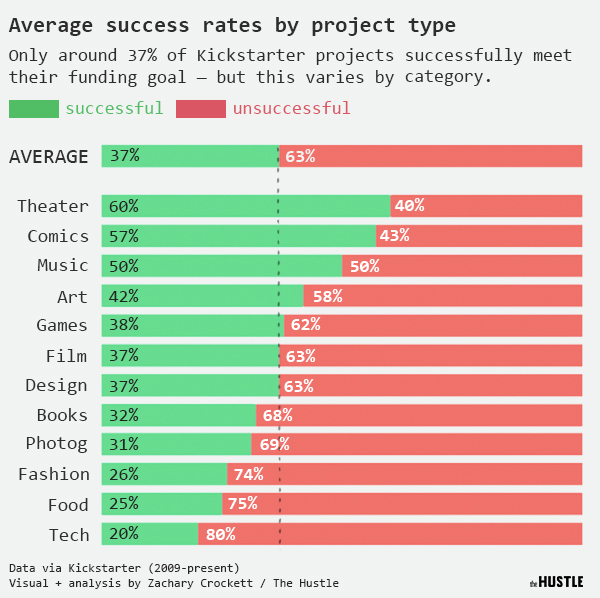
\includegraphics[width=0.6\textwidth]{1/figures/kickstarter_success_rate_2009_2019.jpg}
		\caption{Ratio de éxito de proyectos en Kickstarter desde 2009 hasta 2019 (Febrero). Fuente: \cite{cr_hustle2019successrate}}
		\label{1:fig2}
	\end{center}
\end{figure}


Ya existen estudios previos para predecir la probabilidad de éxito de financiamiento para este tipo de proyectos utilizando técnicas de Aprendizaje Automático. Sin embargo, la mayoría de los modelos predictivos propuestos no arrojan resultados con exactitud muy alta ya que su rango varía entre 60 y 70\%. Esto conlleva a generar imprecisión para pronosticar confiablemente el éxito de financiamiento de estos proyectos de tecnología. Para el presente trabajo de tesis, se creó un modelo predictivo alimentado de datos históricos de la plataforma para estimar el estado final de financiamiento de un proyecto aleatorio, así como su probabilidad de éxito. 



\section{Formulación del Problema}
Para la formulación de los problemas de la presente investigación, se elaboró un «árbol de problemas» (véase Anexo 1).

\subsection{Problema General}
\newcommand{\ProblemaGeneral}{
Bajos niveles de precisión de modelos entrenados de Aprendizaje Automático para cualquier categoría para predecir estado de financiamiento de proyectos de tecnología. 
}
\ProblemaGeneral
\subsection{Problemas Espec\'{i}ficos}
\newcommand{\Pbone}{
Variables de proyectos no normalizadas y varianzas altas.
}
\newcommand{\Pbtwo}{
Datos faltantes o incompletos de proyectos.
}
\newcommand{\Pbthree}{
Parámetros de modelos no ajustados.
}
\newcommand{\Pbfour}{
Sobreajuste de aprendizaje de modelos y clasificación incorrecta de las dos clases del estado final de financiamiento (exitoso o fracasado).
}
\newcommand{\Pbfive}{
Predicción incorrecta de estado de financiamiento de un proyecto tecnológico.
}

\begin{itemize}
	\item \Pbone
	\item \Pbtwo
	\item \Pbthree
	\item \Pbfour
	\item \Pbfive
\end{itemize}

\section{Objetivos de la Investigación}
Para la formulación de los objetivos de la presente investigación, se elaboró un «árbol de objetivos» (véase Anexo 2) 
\subsection{Objetivo General}
\newcommand{\ObjetivoGeneral}{
Construir modelo(s) de Aprendizaje Automático entrenado(s) para predecir correctamente proyectos de tecnología con nivel de precisión aceptable.
}
\ObjetivoGeneral
\subsection{Objetivos Espec\'{i}ficos}
\newcommand{\Objone}{
Normalizar variables de proyectos y reducir niveles altos de varianza.
}
\newcommand{\Objtwo}{
Eliminar datos faltantes o incompletos de proyectos.
}
\newcommand{\Objthree}{
Ajustar parámetros de modelos.
}
\newcommand{\Objfour}{
Evitar sobreajuste de aprendizaje de modelos.
}
\newcommand{\Objfive}{
Predecir correctamente el estado final de financiamiento de cualquier proyecto tecnológico (éxito o fracaso).
}

\begin{itemize}
	\item {\Objone}
	\item {\Objtwo}
	\item {\Objthree}
	\item {\Objfour}
	\item {\Objfive}
\end{itemize}

\section{Justificación de la Investigación}

\subsection{Teórica}
Esta investigación se basa en crear un modelo de Aprendizaje Automático que sea aplicable a proyectos de tecnología de la plataforma Kickstarter por presentar bajas performances en antecedentes.

\subsection{Práctica}
Al culminar la investigación, se ofrecerá un modelo predictivo confiable que ayude a los emprendedores en la toma de decisiones respecto a sus proyectos a partir del insight obtenido de los resultados que deriven a la manipulación de los datos de entrada.

\subsection{Metodológica}
Se creará un modelo predictivo a partir de las variables finales seleccionadas, previa limpieza de datos. Luego, será entrenado y evaluado por las métricas correspondientes. Finalmente, se lanzará una versión de prueba que reciba datos de entrada para predecir la viabilidad de un proyecto de tecnología.

\section{Delimitación del Estudio}

\subsection{Espacial}
Para la presente investigación, se considerará el territorio de los Estados Unidos ya que tanto la campaña del proyecto a servir para la investigación como los datos fuentes de proyectos relacionados financiados previamente, que servirán para la elaboración del modelo predictivo, se encuentran en dicho país.

\subsection{Temporal}
El periodo de tiempo abarcará desde el año 2009, fecha en el cual se tiene registrado los primeros conjuntos de datos de proyectos en Kickstarter hasta el mes de agosto del año 2019, últimos registros descargados hasta el inicio del presente trabajo.

\subsection{Conceptual}
La presente investigación consistirá en la implementación de un modelo predictivo del estado de financiamiento de un proyecto tecnológico en Kickstarter basado en técnicas y conceptos de Aprendizaje Automático, previamente evaluando cuál de todas las existentes genera un mejor desempeño para su uso y análisis de resultados.

\section{Hipótesis}

\subsection{Hipótesis General}
\newcommand{\HipotesisGeneral}{
El modelo entrenado de Aprendizaje Automático logrará predecir correctamente proyectos de tecnología con nivel de precisión aceptable.
}
\HipotesisGeneral
\subsection{Hipótesis Específicas}
\newcommand{\Hone}{
Las variables de los proyectos descargados se normalizarán y se reducirán los niveles altos de varianza.
}
\newcommand{\Htwo}{
Los datos faltantes o incompletos de los proyectos serán eliminados.
}
\newcommand{\Hthree}{
Los parámetros de los modelos usados serán ajustados.
}
\newcommand{\Hfour}{
Se evitará el sobreajuste de aprendizaje de modelos para clasificar correctamente las dos clases del estado final de financiamiento.
}
\newcommand{\Hfive}{
El estado final de financiamiento de cualquier proyecto tecnológico será predicho correctamente.
}
\begin{itemize}
	\item \Hone
	\item \Htwo
	\item \Hthree
	\item \Hfour
	\item \Hfive
\end{itemize}

\subsection{Matriz de Consistencia}
A continuación se presenta la matriz de consistencia elaborada para la presente investigación (véase Anexo \ref{1:table}).

